\documentclass[a4paper,11pt]{book}
\usepackage[margin=2cm]{geometry}		
\usepackage[thinfonts]{uglix2}
\usepackage{array,numprint}
\newcommand{\tabstrut}{\vrule height 1.25em depth 0.5em width 0pt}
\begin{document}
\chapter*{\large Interaction entre l'homme et la machine sur le web \\[-1em]\fontsize{35pt}{42pt}\selectfont Produire un formulaire}
Précédemment nous avons appris à créer des page web dynamiques\\
\double
{
	\begin{enumerate}[--]
		\item 	un fichier \textsc{html} contient la description du contenu;
		\item 	un (éventuel) fichier \textsc{css} contient les éléments de style;
		\item 	un (éventuel) fichier \textsc{JavaScript} contient les scripts qui rendent la page dynamique.
		\item	la page peut utiliser des fichiers multimédias.
	\end{enumerate}
}
{
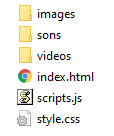
\includegraphics[width=3cm]{img/arborescence_site.png}
}{3cm}

Nous allons maintenant incorporer des \textit{formulaires} dans une page. Un formulaire est un élément d'une page permettant à l'utilisateur de soumettre des données.

\section*{Exemple de formulaire minimal}

Un formulaire est crée à l'aide des balises \htmlinline{<form>} et \htmlinline{</form>}. À l'intérieur de ces balises, il faut indiquer à quoi et comment transmettre les informations collectées. Pour ceci on utilise la balise \htmlinline{<input>} qui n'a pas de balise fermante. Voici un exemple minimaliste de formulaire :

\begin{html}
<!DOCTYPE html>
<html lang="fr">
<head>
    <meta charset="UTF−8">
    <title>Exemple simple</title>
</head>
<body>
<form action="http://monsite.com" method=get>
    <label for="ChampNomEleve">Nom de l'élève :</label> 
    <input id="ChampNomEleve" name="nomEleve" type="text">
</form>
</body>
</html>
\end{html}

Dans la balise \htmlinline{<form>} on indique que le formulaire doit être renvoyé à l'adresse \url{http://monsite.com}, avec la méthode \tw{get}. Ce 
site n'existe pas (ou bien s'il existe nous n'en sommes pas propriétaire et ne pouvons donc pas le modifier) et nous verrons plus tard ce qu'est la 
méthode \tw{get}.\\
Passons en revue ce code : d'abord on crée un label pour l'objet qui a l'\tw{id} \tw{ChampNomEleve}. Cet objet est un \htmlinline{<input>} de type 
\tw{text} car on attend que l'utilisateur entre du texte, et la variable à laquelle on affectera la valeur entrée s'appelle \tw{nomEleve}


\begin{exercice}[]
Le formulaire précédent est accessible sous le nom \tw{exemple\_formulaire.html}. \'Execute-le. Que peut-on reprocher à ce petit formulaire (hormis 
le fait qu'il appelle une page qui n'existe pas)?
\end{exercice}

\section*{À toi de jouer}

On aimerait créer le formulaire suivant (pas de fioritures, pas de \textsc{CSS} ni de \textsc{JavaScript}):
\begin{center}
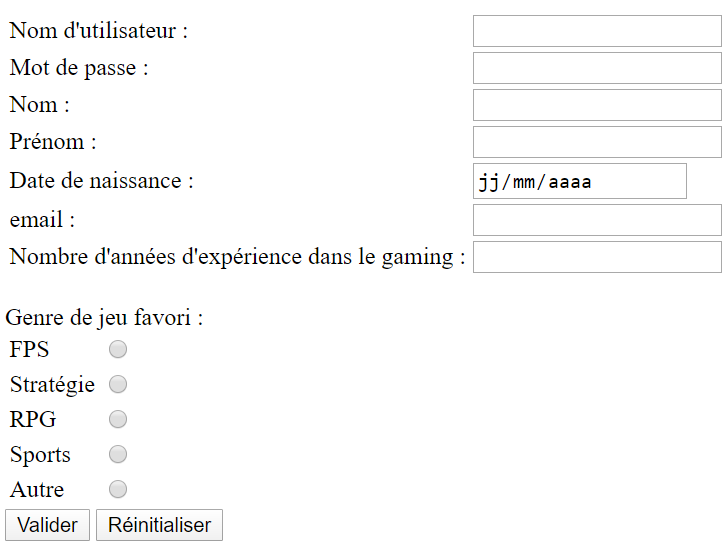
\includegraphics[width=12cm]{img/formulaire.png}
\end{center}

Avec les contraintes suivantes :
\begin{enumerate}[--]
	\item 	Le mot de passe doit être caché quand on l'entre;
	\item 	On doit pouvoir sélectionner la date dans un calendrier qui s'affiche quand on clique dans le champ approprié;
	\item 	L'email doit comporter un \url{@};
	\item 	Le nombre d'années d'expérience doit être un nombre;
	\item 	On ne peut choisir qu'un genre de jeu favori;
	\item 	On ne peut valider que quand tous les champs sont remplis.
\end{enumerate}

\begin{exercice}[]
En t'aidant de la page \url{https://www.w3schools.com/tags/att_input_type.asp} (et éventuellement d'autres sources), construis un tel formulaire :
\begin{enumerate}[--]
	\item 	Il faudra utiliser plusieurs \textit{types} de \htmlinline{<input>};
	\item 	Pour que ce soit joli tu peux placer les éléments dans une \htmlinline{<table>};
	\item 	Pour l'instant, on ne cherche pas vraiment à soumettre le formulaire, donc tu peux recopier la ligne 
			\htmlinline{<form action="http://monsite.com"  method=get>}.
\end{enumerate}

\end{exercice}

\section*{Les méthodes \tw{get} et \tw{post}}


\begin{exercice}[]
Lorsque tu valides ton formulaire, le navigateur essaie d'accéder à un site qui n'existe pas, donc il y a une erreur.\\
Cependant examines la barre d'adresse. Que reconnais-tu ?\\

Change la ligne avec la balise \htmlinline{<form>} en :\\
\htmlinline{<form action="http://monsite.com"  method=post>}\\ et recommence. Que constates-tu ?
\end{exercice}

\begin{enumerate}[--]
	\item 	La méthode \tw{get} inclut toutes les informations du formulaire dans l'\textsc{url} (l'adresse) auquel le formulaire soumet ces informations;
	\item 	La méthode \tw{post} inclut également ces informations mais elles sont à l'intérieur de la requête \textsc{http}, et pas dans l'\textsc{url}.
\end{enumerate}

\section*{Vous reprendrez bien un peu de JS}

Le problème de ce formulaire, c'est qu'on peut entrer à peu près n'importe quel mot de passe.
Comment pourrait-on remédier à ce problème ?
\end{document}